
\clearpage
\section{Transactions}

The 'Transactions' part of CUBE PA supports the management of a structured project journal. The project journal consists of a collection of transactions which in turn are divided into subtransactions. The number of subtransactions is unlimited. A chronology for each subtransaction is available in CUBE PA. The most recent entry is displayed at the top.

\vspace{\baselineskip}

The philosophy behind the transaction and subtransaction structure can be explained with the following example: You are promoted to director and mus therefore dress accordingly. The transaction 'buy business suits' can be divided into a number of subtransactions: go to color advice, market research on the most important online offers, buy suits, buy shirts, buy shoes, etc. Once all subtransactions are complete, the transaction is also complete.

\vspace{\baselineskip}

A history is recorded within each subtransaction in the form of entries. The entries basically correspond to the rows of an Excel table. The idea is to record all processes relevant to the project journal in the form of entries. CUBE PA displays the entries in chronological order, with the most recent entry at the top.

\subsection{Creating a transaction}

\begin{wrapfigure}[3]{l}{6.5cm}   % [x] Wie manche Zeile soll sich um die Grafik "brechen"
  \vspace{-35pt}      % Grundwert war 20; mit 30 schön oben beim Text ausgerichtet
  \begin{center}
    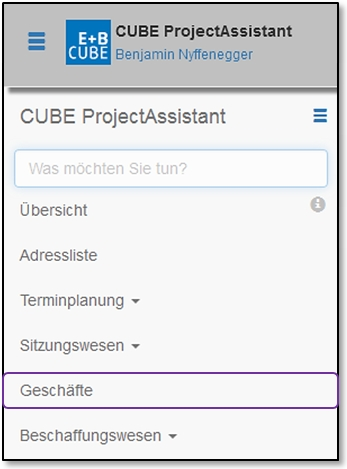
\includegraphics[width=1\linewidth]{../chapters/06_Geschaefte/pictures/6-1_Menu_Geschaefte.jpg}
  \end{center}
  \vspace{-20pt}
  \caption{Organizing transactions and contracts}
  \vspace{-10pt}
\end{wrapfigure}

Select the 'Transactions' menu item from the menu on the left. \\

\vspace{6cm}

\pagebreak

The list of transactions appears:

\begin{figure}[H]
\center{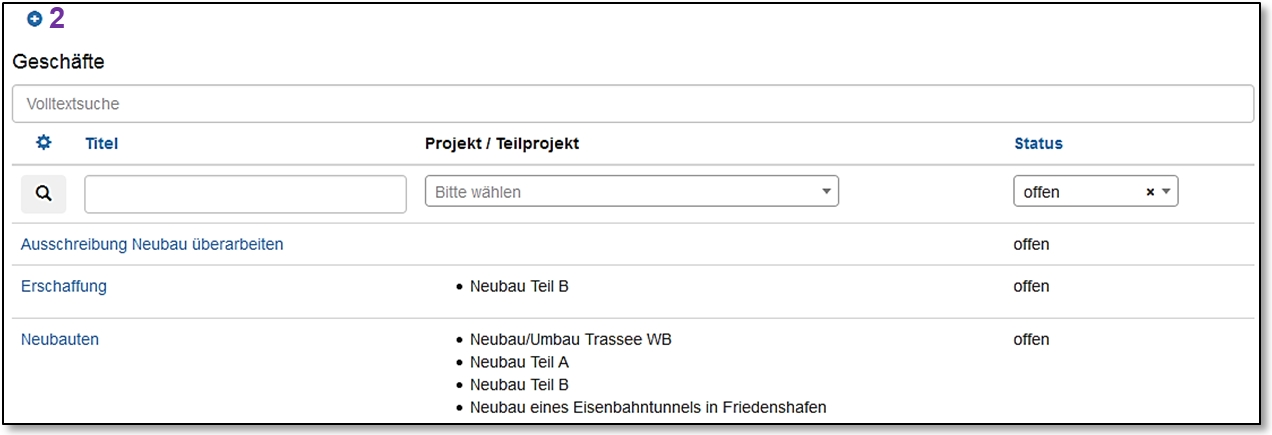
\includegraphics[width=1\linewidth]{../chapters/06_Geschaefte/pictures/6-1_GeschaefteUebersicht.jpg}}
\caption{Overview of the transactions}
% \label{fig:speciation}
\end{figure}

Click on the plus sign 
\includegraphics[height=12pt]{/Icons/Plussymbol.jpg} \col{(2)} on the top left and the form for creating a new transaction appears.

\begin{figure}[H]
\center{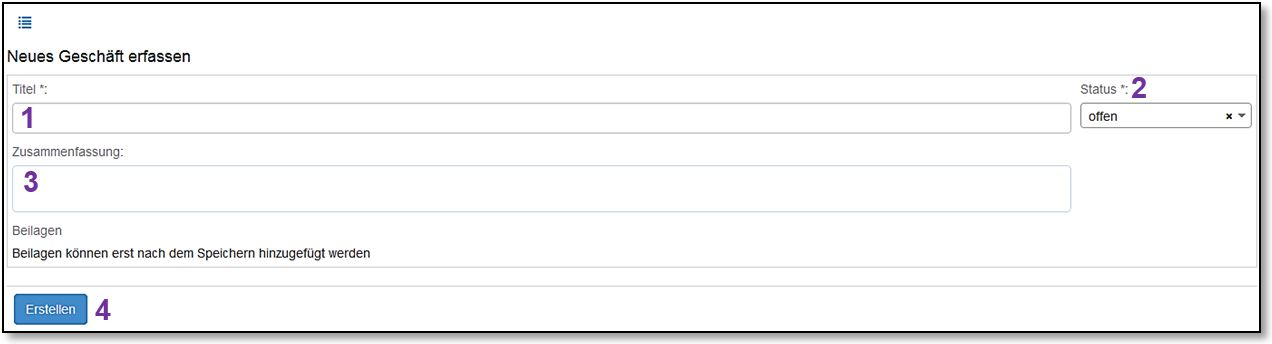
\includegraphics[width=1\linewidth]{61_NeueGeschaefteErfassen.jpg}}
\caption{Creating new transactions}
% \label{fig:speciation}
\end{figure}

Mandatory fields are marked with an asterisk *.

\begin{itemize}
\item
Title \col{(1)}: Enter the name of the transaction as free text.
\item 
Status \col{(2)}: There are only the statuses 'open' and 'complete'. The first is set when creating a new transaction, and the second can be set when the transaction is complete.
\item
Summary \col{(3)}: Describe the transaction in two to three lines of free text.
\end{itemize}

Click the 'Create' button 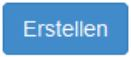
\includegraphics[height=12pt]{/Icons/B_Erstellen.jpg} \col{(4)}, and you'll have the option to upload attachments.

\begin{figure}[H]
\center{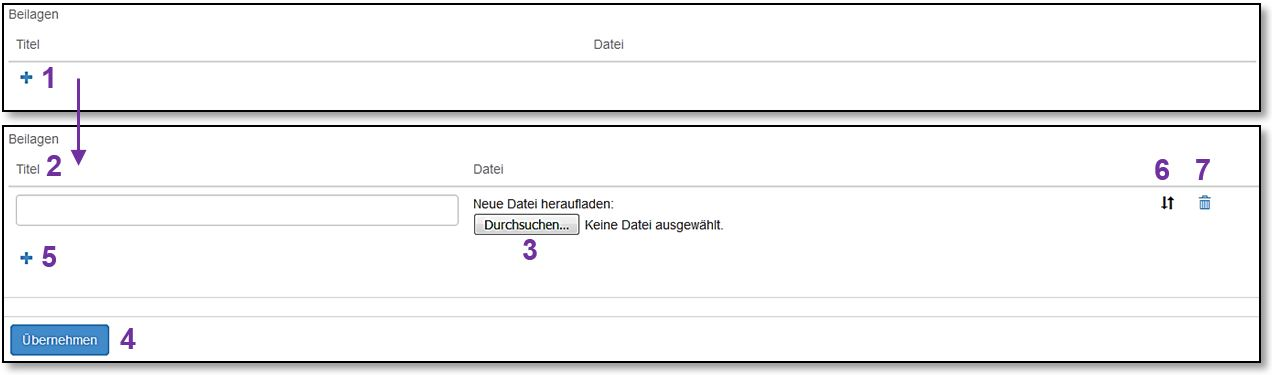
\includegraphics[width=1\linewidth]{61_GeschaefteBeilagenHochladen.jpg}}
\caption{Uploading attachments}
% \label{fig:speciation}
\end{figure}

Uploading attachments is mainly intended to avoid entering long explanations. You therefore have the option to refer to an attachment.

\vspace{\baselineskip}

To add an attachment, click on the plus sign 
\includegraphics[height=12pt]{/Icons/Pluszeichen.jpg} \col{(1)}. The fields for uploading an attachment appear:

\begin{itemize}
\item
Title \col{(2)}: Give an suitable name for the attachment.
\item
To upload a document, click on the 'Search' button \col{(3)} and double click on the desired document. If you uploaded the wrong file, simply upload a new one.
\item
Then click on the 'Apply' button \col{(4)} and the attachment is added.
\end{itemize}


You can add as many attachments as needed by clicking on the plus sign 
\includegraphics[height=12pt]{/Icons/Pluszeichen.jpg} \col{(5)}. You can change the order of the attachments by dragging the symbol with vertical opposing arrows 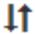
\includegraphics[height=12pt]{/Icons/VertPfeile.jpg} \col{(6)} and dropping it at the desired position. Clicking on the garbage bin symbol 
\includegraphics[height=12pt]{/Icons/Muelltonne.jpg} \col{(7)} removes an attachment.

% bishierher

\subsection{Creating a subtransaction}

You can either go to the same screen as when adding attachments to a transaction, or you can go back to the menu and select the 'Transactions' item. In the list of transactions you can select the transaction for which you want to create a subtransaction.

\vspace{\baselineskip}

You can now search optically within the entire list of transactions or filter through the list. To search through the list of transactions simply scroll down to the pagination. You can switch pages by clicking on the page numbers or using the 'Next' and 'Previous' buttons.

\begin{center}

\includegraphics[height=12pt]{/Icons/SeitenBlaettern.jpg}
\end{center}

You can use the search fields to filter through the list or a separate field for a full text search \col{(1)}. In the 'Title' field \col{(2)} you can enter free text. For the 'Project/Subproject' field \col{(3)} and the 'Status' field \col{(4)} there's a selection list. Once you have selected the filter values, click on the magnifying glass symbol 
\includegraphics[height=12pt]{/Icons/Lupe_kl.jpg} \col{(5)} on the left (or hit 'Enter') and the filtered list appears. Alternatively, you can use the full text search to search for keywords in the list. Click on the magnifying glass symbol 
\includegraphics[height=12pt]{/Icons/Lupe_kl.jpg} \col{(5)} or hit 'Enter' to start the search.

\begin{figure}[H]
\center{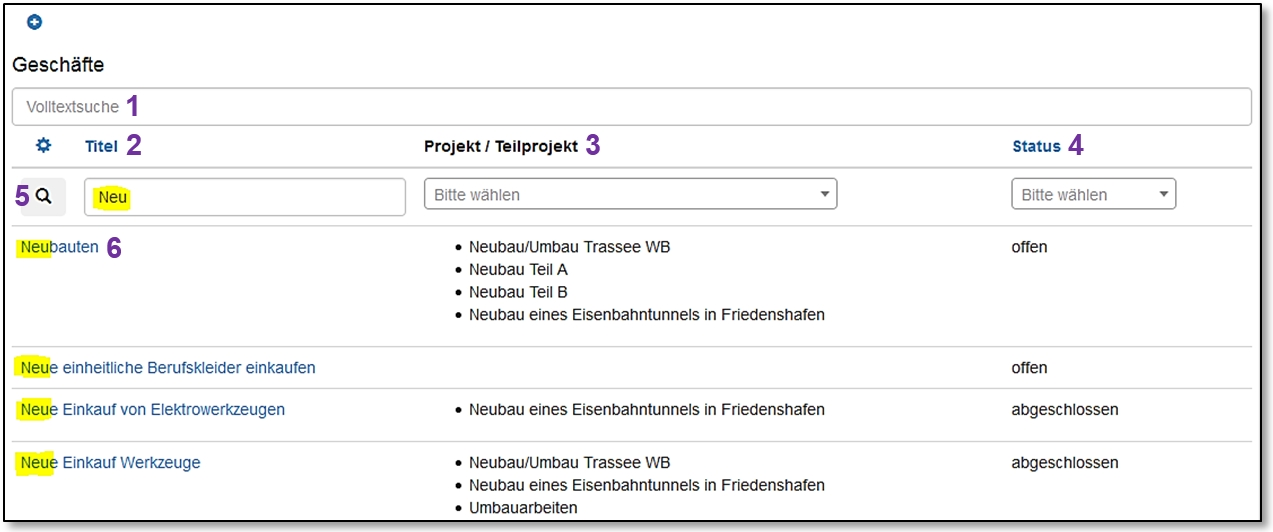
\includegraphics[width=1\linewidth]{../chapters/06_Geschaefte/pictures/6-2_FilterAnwenden.jpg}}
\caption{Using the filter}
% \label{fig:speciation}
\end{figure}

When you find the relevant transaction, click on the blue title text of the transaction \col{(6)}. The form with an overview of the transaction appears.

\begin{figure}[H]
\center{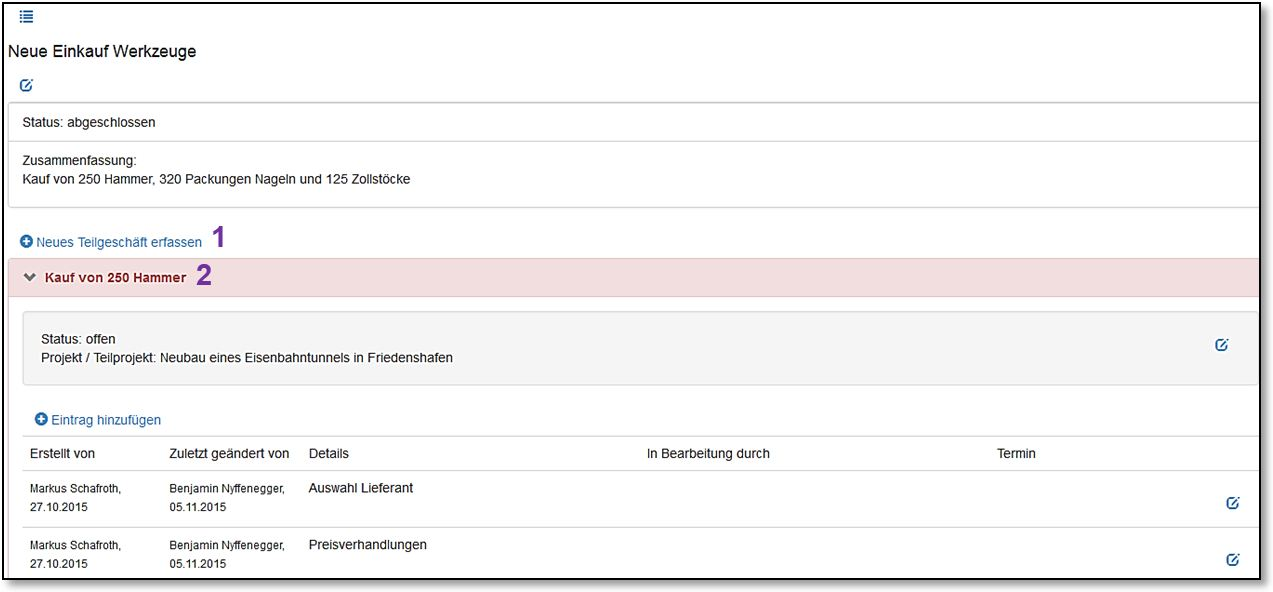
\includegraphics[width=1\linewidth]{62_GeschaefteUebersicht.jpg}}
\caption{Overview of the transactions}
% \label{fig:speciation}
\end{figure}

Below the title, the status, the summary and the attachments you will find a plus sign 
\includegraphics[height=12pt]{62_TeilgeschaeftErfassen.jpg} \col{(1)} with which you can create a new subtransaction. Existing subtransactions are shown below it \col{(2)}.

\vspace{\baselineskip}

Click on 'Create new subtransaction' and a window is opened in which you can enter the information about the subtransaction.

\begin{figure}[H]
\center{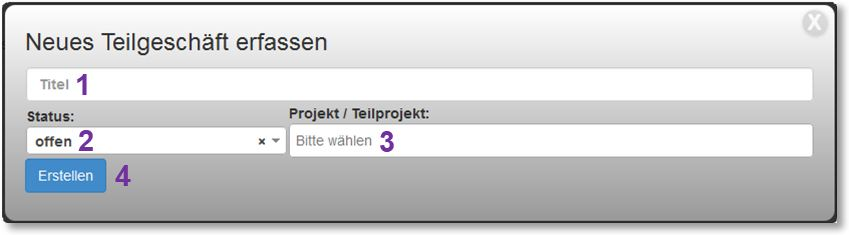
\includegraphics[width=0.5\linewidth]{62_NeuesTeilgeschaeftErfassen.jpg}}
\caption{Creating a new subtransaction}
% \label{fig:speciation}
\end{figure}

Enter the required information in the fields:

\begin{itemize}
\item
'Title' \col{(1)} allows the input of free text.
\item
'Status' \col{(2)} is automatically set to 'open'. When the subtransaction is complete, you can set the status to 'complete'.
\item
The 'Project/Subproject' field \col{(3)} contains a selection list from which you can link the subtransaction to a project or a subproject. The transaction to which the subtransaction is subordinated inherits this link. It is shown in the list of the transaction. The transaction inherits the sum of all (sub)projects assigned to its subordinate subtransactions.
\end{itemize}

Click on the 'Create' button \col{(4)} to save the subtransaction. The title of the subtransaction only appears in the pink rectangle in the overview of the transaction. You now have the possibility to either add an entry to the new subtransaction or to add another subtransaction. If you enter more than one subtransaction, the latest one appears at the top in the overview.

\subsection{Accessing the overview of a transaction}

If you want to have a complete overview of a transaction, select the 'Transactions' menu item. In the list of transactions, look for the transaction whose overview you need.

\begin{figure}[H]
\center{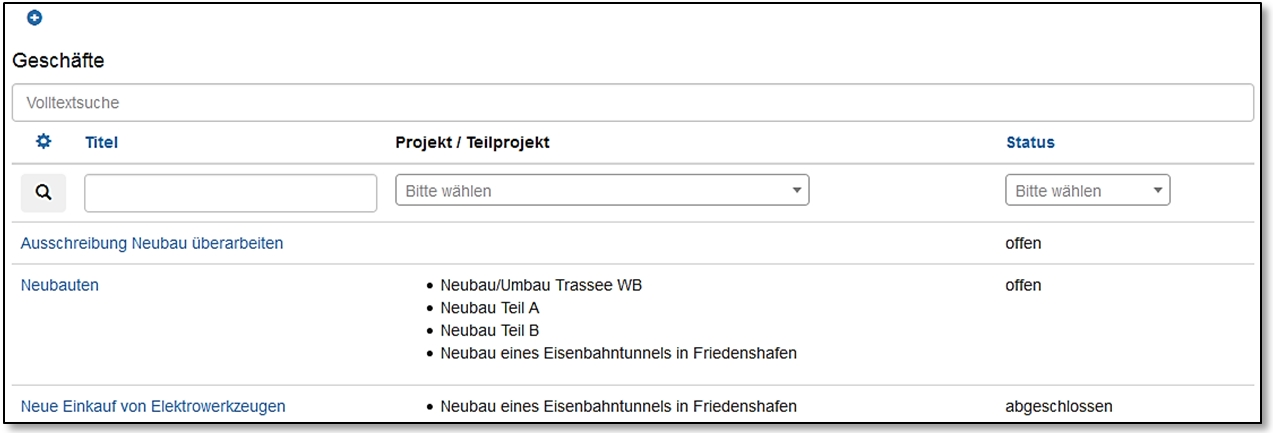
\includegraphics[width=1\linewidth]{../chapters/06_Geschaefte/pictures/6-3_UeberblickGeschaeft.jpg}}
\caption{Overview of transactions}
% \label{fig:speciation}
\end{figure}

You can now search optically within the entire list of transactions or filter through the list. To search through the list of transactions simply scroll down to the pagination. You can switch pages by clicking on the page numbers or using the 'Next' and 'Previous' buttons.

\begin{center}

\includegraphics[height=12pt]{/Icons/SeitenBlaettern.jpg}
\end{center}

You can use the search fields to filter through the list. In the 'Title' field \col{(1)} you can enter free text. For the 'Project/Subproject' field \col{(2)} and the 'Status' field \col{(3)} there's a selection list. Once you have selected the filter values, click on the magnifying glass symbol 
\includegraphics[height=12pt]{/Icons/Lupe_kl.jpg} \col{(4)} on the left (or hit 'Enter') and the filtered list appears.

\begin{figure}[H]
\center{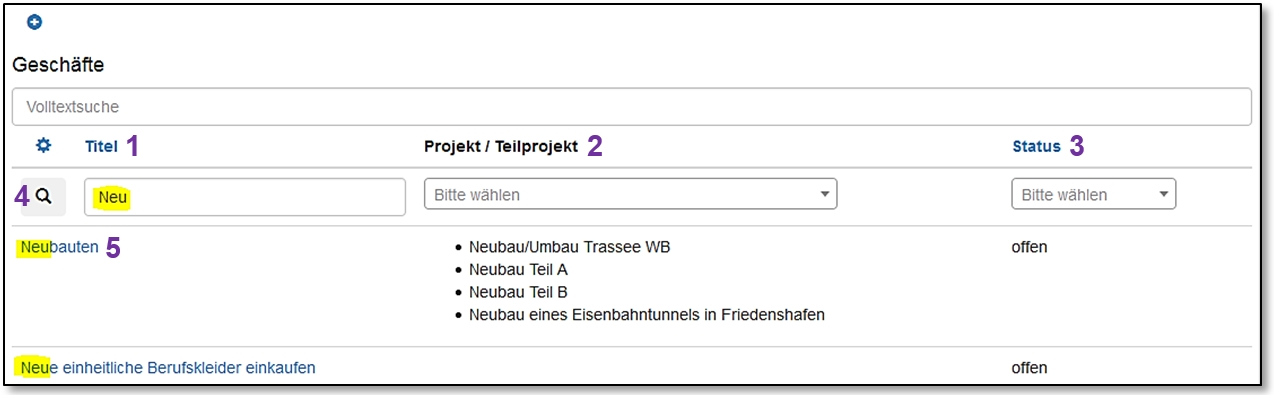
\includegraphics[width=1\linewidth]{../chapters/06_Geschaefte/pictures/6-3_GeschaefteFiltern.jpg}}
\caption{Filtering transactions}
% \label{fig:speciation}
\end{figure}

When you find the relevant transaction, click on the blue title text of the transaction \col{(5)}. The form with an overview of the transaction appears.

\begin{figure}[H]
\center{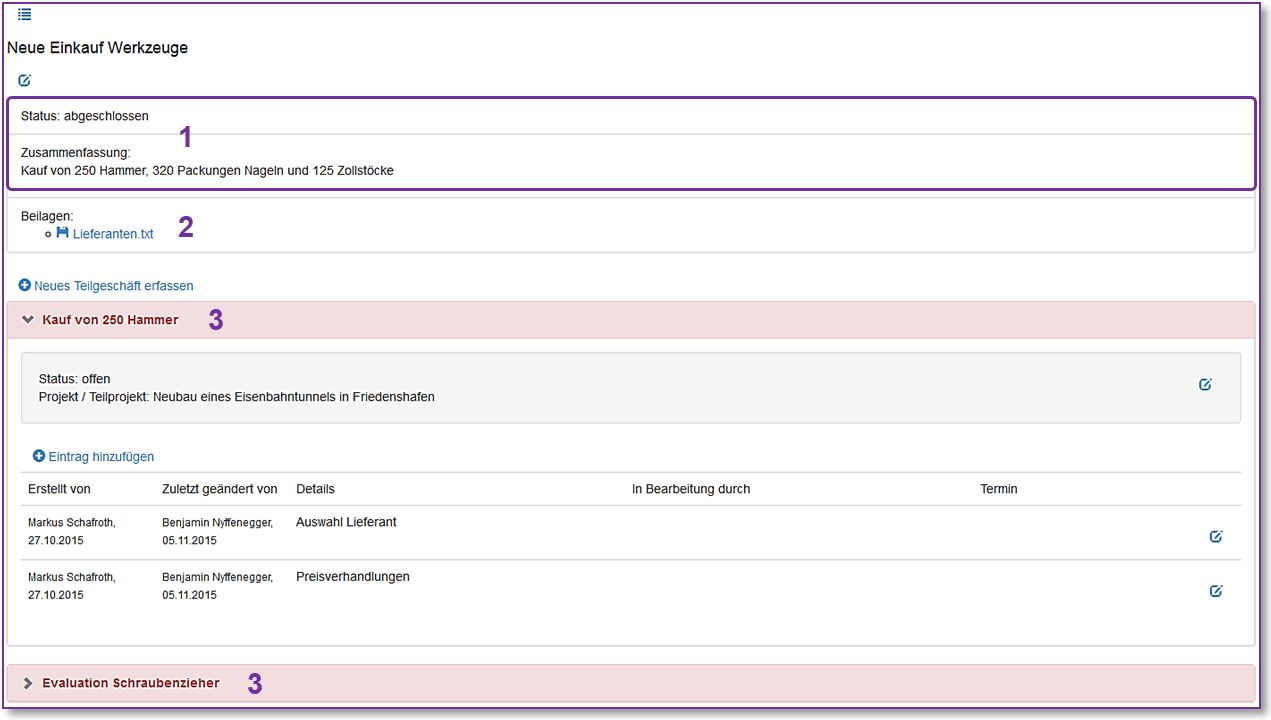
\includegraphics[width=1\linewidth]{63_Geschaeftsuebersicht.jpg}}
\caption{Overview of a transaction}
% \label{fig:speciation}
\end{figure}

In this overview you will find the general information about the transaction \col{(1)} and below the list of attachments \col{(2)}, if there are any. Further below, the subtransactions \col{(3)} are listed, with each title in a pink rectangle.

\vspace{\baselineskip}

Select a subtransaction and click on the arrow 
\includegraphics[height=12pt]{/Icons/Pfeil_rechts_rosa.jpg} left of the title. Its direction changes from horizontal to vertical 
\includegraphics[height=12pt]{/Icons/Pfeil_unten_rosa.jpg} and the contents of the subtransaction are now displayed. Above you will find the general information about the subtransaction, and below the entries with the most recent one at the top.

\vspace{\baselineskip}

Repeat this for all subtransactions and you will have the overview of all the entries of all the subtransactions of the transaction.

\begin{figure}[H]
\center{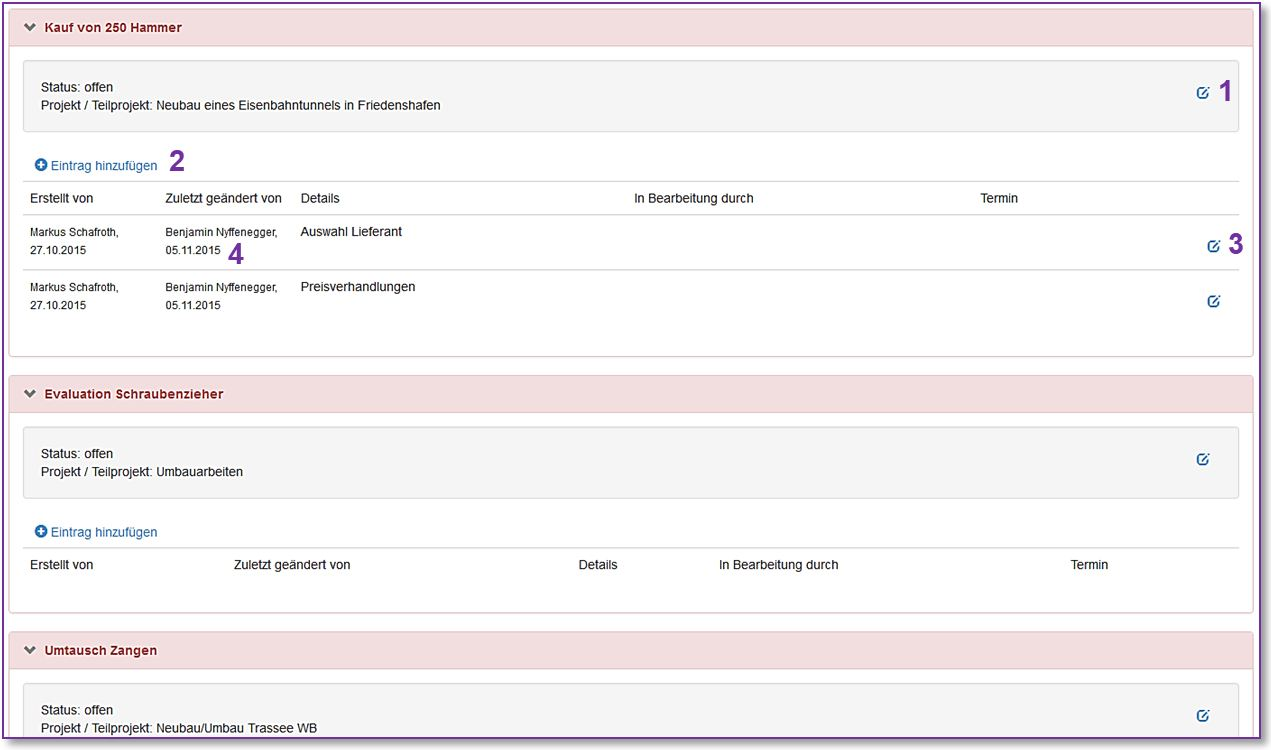
\includegraphics[width=1\linewidth]{63_UeberblickTeilgeschaefte.jpg}}
\caption{Overview of subtransactions}
% \label{fig:speciation}
\end{figure}

The pen symbol 
\includegraphics[height=12pt]{/Icons/Bearbeiten.jpg} \col{(1)} on the right of the general information of a subtransaction enables you to edit it.

\subsection{Adding entries to subtransactions}

You can add an entry to a subtransaction either directly after creating the subtransaction or at any time after that, by searching for the subtransaction and displaying its content as explained previously.

Click on 'Add Entry' 
\includegraphics[height=12pt]{64_TeilgeschaefteEintragHinzufuegen.jpg} \col{(1)} under the gray field with the general information about the subtransaction. The window for adding an entry appears.

\begin{figure}[H]
\center{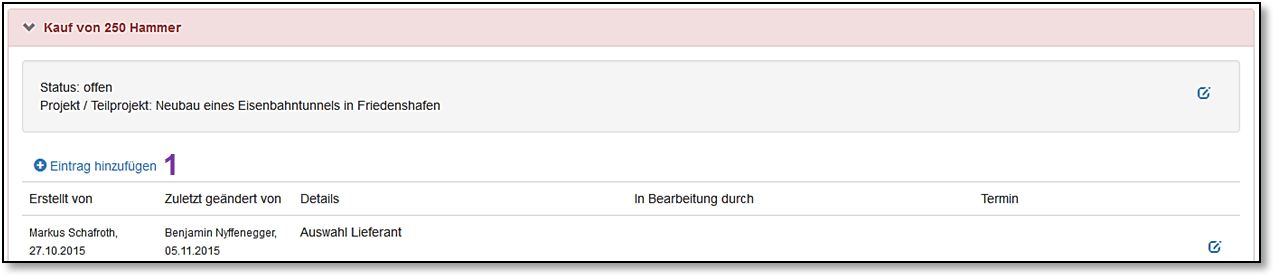
\includegraphics[width=1\linewidth]{64_TeilgeschaefteEintragHinzufuegenMaske.jpg}}
\caption{Overview of the subtransaction}
% \label{fig:speciation}
\end{figure}

\begin{figure}[H]
\center{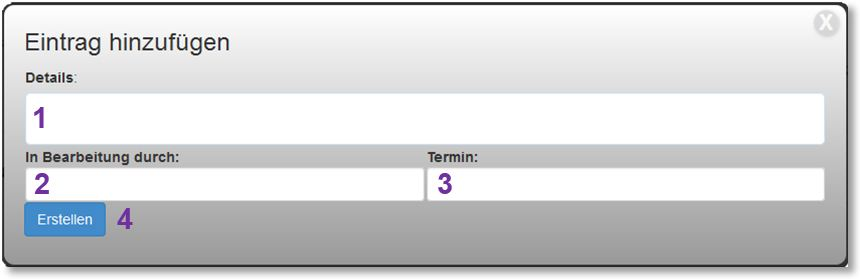
\includegraphics[width=.75\linewidth]{64_TeilgeschaefteHinzufuegenFelder.jpg}}
\caption{Adding an entry to a subtransaction}
% \label{fig:speciation}
\end{figure}

Fill out the fields:

\begin{itemize}
\item
'Details' \col{(1)} is a free text field for describing an entry, e.g. the description of a process.
\item
'Processed by' \col{(2)} is a free text field for entering who will process the task described in the entry.
\item
'Due date' \col{(3)} should be filled out in date format DD.MM.YYYY. This allows you to specify when the task described in the entry is to be completed.
\item
If the entry only describes a statement for example, the 'Processed by' and 'Due date' fields don't need to be filled.
\end{itemize}

Click on the 'Create' button \col{(4)} and the entry appears in the overview of the subtransaction.

\begin{figure}[H]
\center{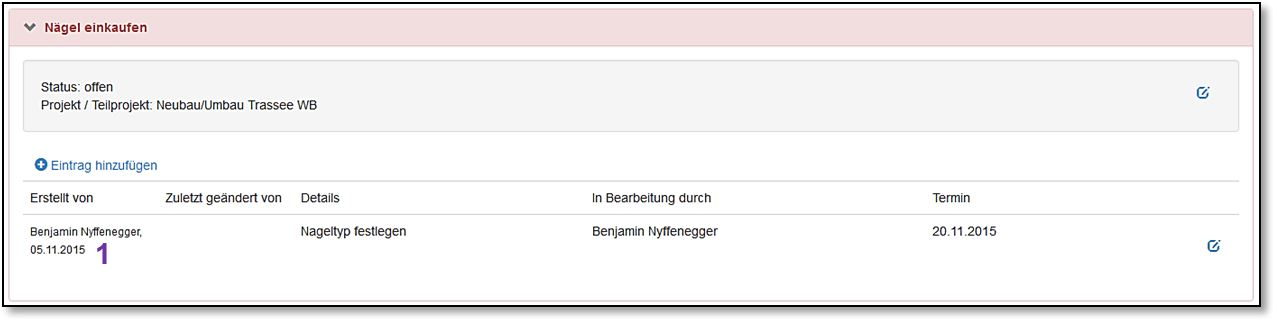
\includegraphics[width=1\linewidth]{64_TeilgeschaeftErstellen.jpg}}
\caption{Subtransaction overview}
% \label{fig:speciation}
\end{figure}

On the left on the entry, the date the entry was added and the author of the entry \col{(1)} are visible. This helps the reader of an entry to situate the entry in time and to ask questions about the entry.

If there are more than one entry for a subtransaction, these appear in reverse chronological order (most recent entry at the top).

\subsection{Editing existing entries}

To edit an existing entry, first display the overview of the relevant transaction and its subtransactions as described above. Display the entries of the subtransaction by clicking on the arrow 
\includegraphics[height=12pt]{/Icons/Pfeil_rechts_rosa.jpg} on the left of the title.
	
\begin{figure}[H]
\center{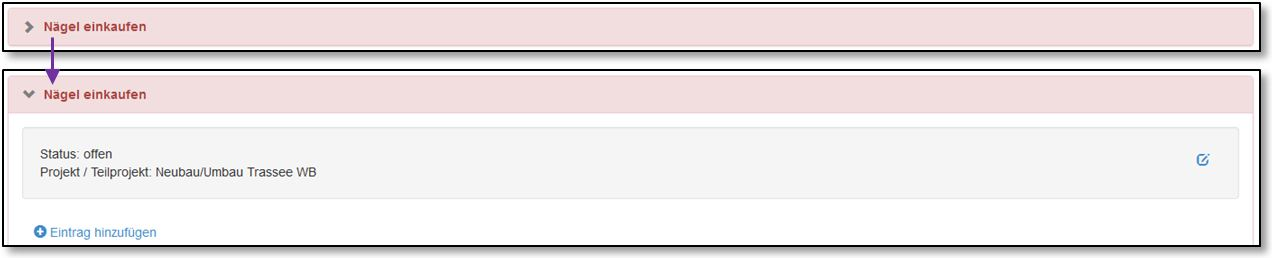
\includegraphics[width=1\linewidth]{65_GeschaefteDetails.jpg}}
\caption{Subtransactions: Show details}
% \label{fig:speciation}
\end{figure}

All entries for the selected subtransaction are shown in reverse chronological order (most recent entry at the top).

\begin{figure}[H]
\center{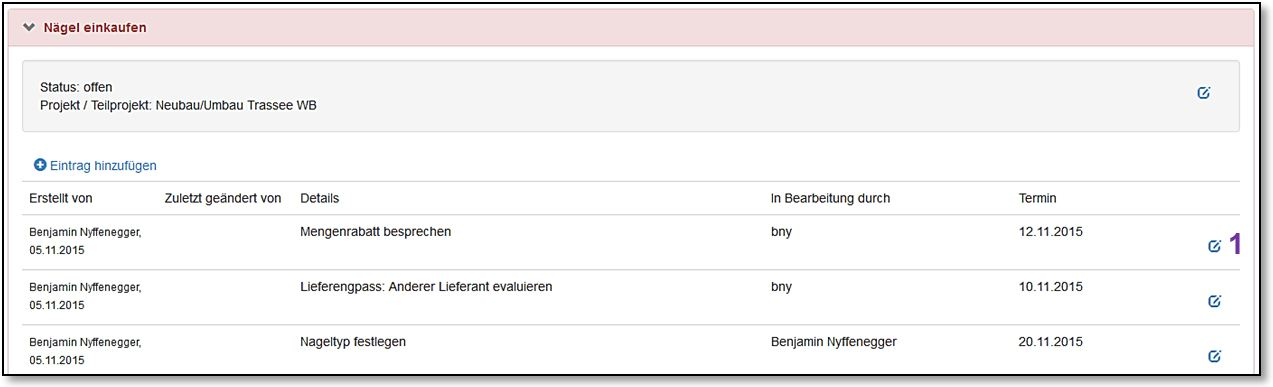
\includegraphics[width=1\linewidth]{65_GeschaefteEintraege.jpg}}
\caption{Subtransactions: Show all entries}
% \label{fig:speciation}
\end{figure}

Scroll through the entries to find the one you want to edit.

\vspace{\baselineskip}

Click on the pen symbol 
\includegraphics[height=12pt]{/Icons/Bearbeiten.jpg} \col{(1)} on the right in the entry and a window for editing the entry appears.

\begin{figure}[H]
\center{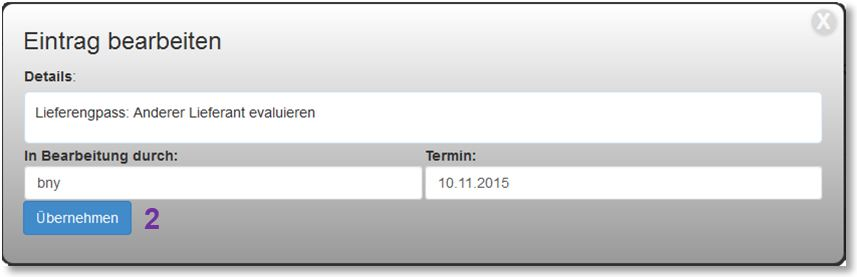
\includegraphics[width=.75\linewidth]{65_GeschaefteEintraegeBearbeiten.jpg}}
\caption{Subtransactions: Editing entries}
% \label{fig:speciation}
\end{figure}

Make your changes in the fields then click on 'Apply' \col{(2)}. The modified entry now appears in the list of entries. On the left, next to the date the entry was added and its author, the date the entry was modified appears along with the name of the user who made the changes \col{(3)}.

\begin{figure}[H]
\center{
\includegraphics[width=1\linewidth]{65_GeschaefteEintraegeNachverf.jpg}}
\caption{Subtransactions: Tracking changes}
% \label{fig:speciation}
\end{figure}

\textbf{Note}: The content of the changes is not logged, that is only the latest field contents are saved.

\vspace{\baselineskip}

\textbf{Note}: When an entry is modified more than once, only the date the entry was added, the name of the author, the date it was last modified, and the name of the user who made the last changes are saved. Information about the previous changes is lost.

\subsection{Editing general information of a transaction}

Select the 'Transactions' menu item and search for the relevant transaction in the list of transactions, either by browsing the list optically or by filtering through the list. Click on the blue title of the desired transaction. The transaction is opened with a the detailed view:

\begin{figure}[H]
\center{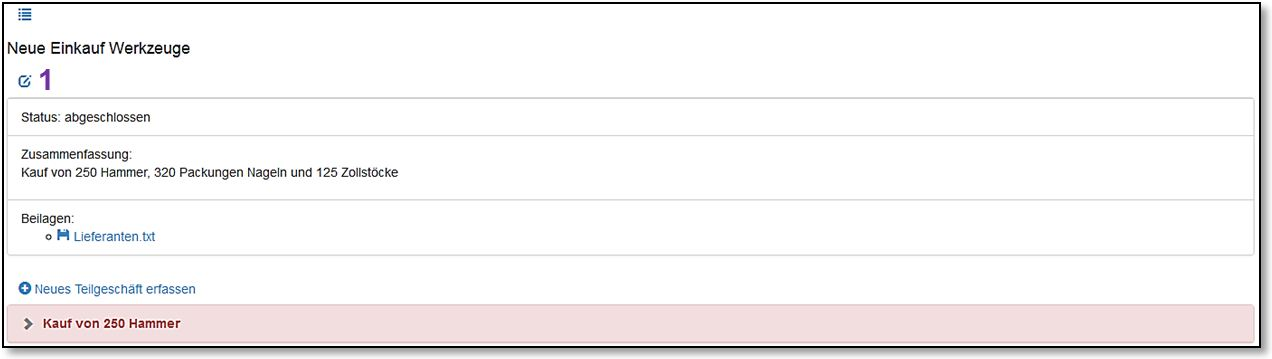
\includegraphics[width=1\linewidth]{66_GeschaefteEintragUeberblick.jpg}}
\caption{Transaction overview}
% \label{fig:speciation}
\end{figure}

Click on the pen symbol 
\includegraphics[height=12pt]{/Icons/Bearbeiten.jpg} \col{(1)} under the title of the transaction.

\begin{figure}[H]
\center{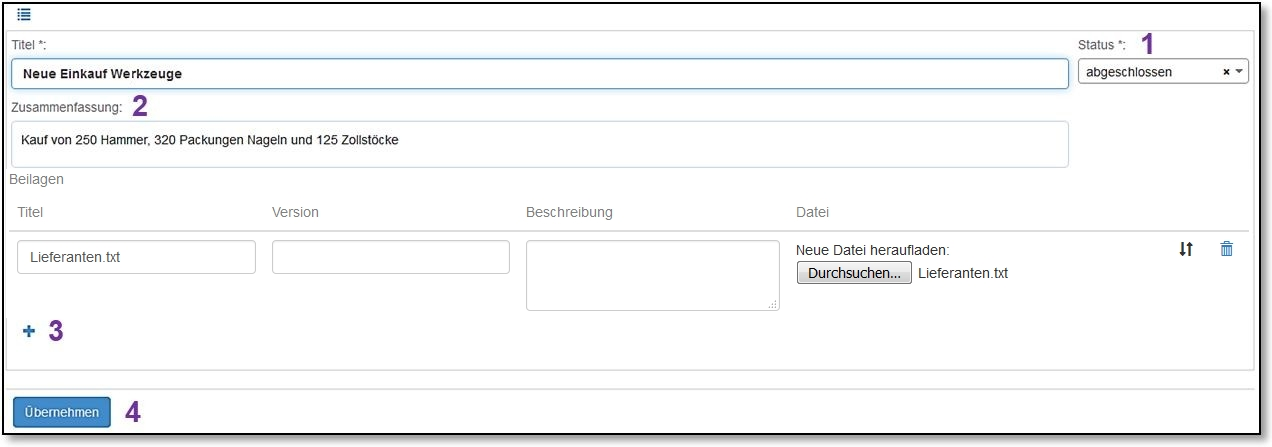
\includegraphics[width=1\linewidth]{../chapters/06_Geschaefte/pictures/6-6_GeschaefteEintragBearbeiten.jpg}}
\caption{Editing a transaction}
% \label{fig:speciation}
\end{figure}

Now you can edit the contents of the 'Status' field \col{(1)} and the 'Summary' field \col{(2)}, as well as upload attachments \col{(3)}. Click on 'Apply' \col{(4)} to back up the data.

\subsection{Editing general information of a subtransaction}

Open the overview of the relevant transaction and its corresponding subtransactions as described above. Display the contents of the subtransaction by clicking on the arrow 
\includegraphics[height=12pt]{/Icons/Pfeil_rechts_rosa.jpg} on the left next to the title. Unde the title a gray field \col{(1)} is displayed with the general content of the subtransaction.

\begin{figure}[H]
\center{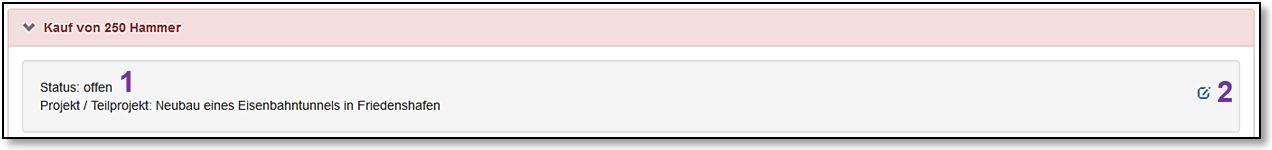
\includegraphics[width=1\linewidth]{67_Teilgeschaeft.jpg}}
\caption{Subtransaction overview}
% \label{fig:speciation}
\end{figure}

Click on the pen symbol 
\includegraphics[height=12pt]{/Icons/Bearbeiten.jpg} \col{(2)} on the right in this field. The window for editing the general information of the subtransaction appears.

\begin{figure}[H]
\center{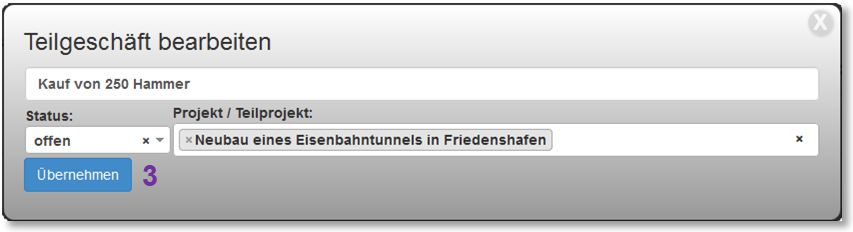
\includegraphics[width=.75\linewidth]{67_TeilgeschaeftBearbeiten.jpg}}
\caption{Editing a subtransaction}
% \label{fig:speciation}
\end{figure}

You can now edit the contents of the fields. Clicl on 'Apply' \col{(3)} to back up the data.
